% !TeX root = ../main.tex

\section{简介}

\begin{frame}{\TeX 与 \LaTeX}
  \begin{columns}[T]
    \column{.8\textwidth}
    \begin{itemize}
      \item \TeX: $\tau\varepsilon\chi$ (
        \textipa{/tEx/}
        \footnote{\textipa{/x/}为软腭清擦音,不读作\textipa{/ks/},类似汉语拼音中的\textipa{h}\\
        图片来源:
          \link{https://www-cs-faculty.stanford.edu/~knuth/graphics.html}
          \link{https://www.quantamagazine.org/computing-expert-says-programmers-need-more-math-20220517}
        },
        \textipa{/tEk/}
      )
        \begin{itemize}
          \item 生成精美图书的排版系统
          \item 最初由 高德纳 \zhparen{Donald E. Knuth} 于 1978 年开发用于其著作《计算机程序设计艺术》
          \item 漂亮、美观、稳定、通用
          \item 尤其擅长数学公式排版
        \end{itemize}
      \item \LaTeX\ (\textipa{/'la:tEx/}, \textipa{/'leItEk/})
        \begin{itemize}
          \item Leslie Lamport 开发的一种 \TeX{} 格式
          \item 在 \TeX 的基础上提供宏包, 降低使用门槛
          \item 极其丰富的宏包,提供扩展功能
          \item 广泛用于学术界,期刊会议论文模板
          \item 大学学位论文模板,如 \pkg{hustthesis}
        \end{itemize}
    \end{itemize}
    \column{.2\textwidth}
    \vspace*{0.05\paperheight}
    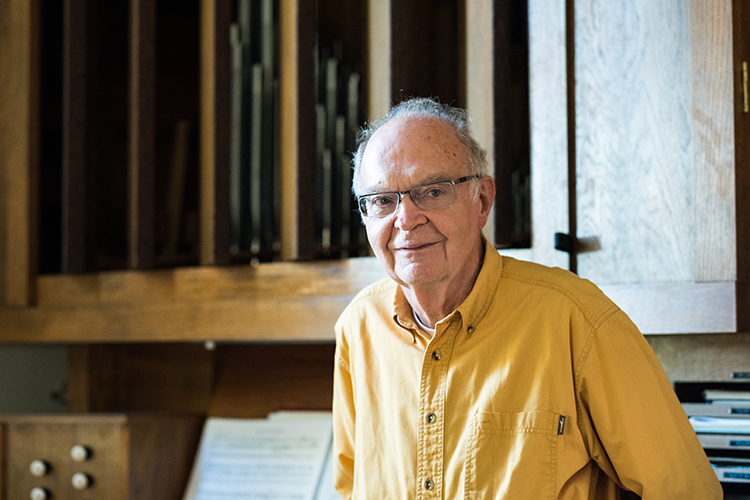
\includegraphics[width=\textwidth]{Knuth-2018.jpg}

    \vspace*{0.18\paperheight}
    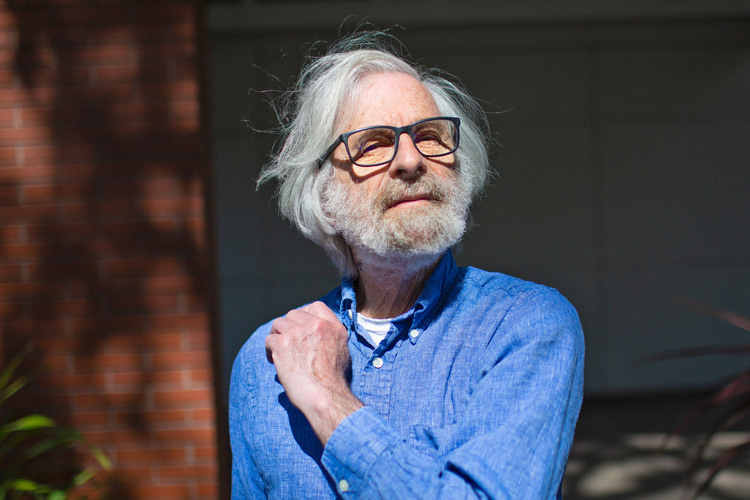
\includegraphics[width=\textwidth]{Lamport-2022.jpg}

  \end{columns}
\end{frame}

\begin{frame}{和 Word 对比}
  注:术业有专攻,评价需客观
  \begin{table}[h]
    \centering
    \rowcolors[]{1}{hustblue!20}{hustblue!40}
    \begin{tabular}{c|c}
      Microsoft\textsuperscript{\textregistered} Word & \LaTeX \\
      \hline
      字处理工具 & 专业排版软件 \\
      容易上手,简单直观 & 容易上手 \\
      所见即所得 & 所见即所想,所想即所得 \\
      高级功能不易掌握 & 进阶难,但一般用不到 \\
      处理长文档需要丰富经验 & 和短文档处理基本无异 \\
      花费大量时间调格式 & 无需担心格式,专心作者内容 \\
      公式排版差强人意 & 尤其擅长公式排版 \\
      二进制格式,兼容性差 & 文本文件,易读、稳定 \\
      付费商业许可 & 自由免费使用 \\
    \end{tabular}
  \end{table}
\end{frame}

\begin{frame}{\TeX{}排版举例:公式}
  \begin{exampleblock}{无编号公式}
    \begin{equation*}
      \mathcal{F}(\xi)=\int_{-\infty}^{\infty} f(x)\mathrm{e}^{-\mathrm{j}2\pi \xi x}\,\mathrm{d}x
    \end{equation*}
  \end{exampleblock}
  \begin{exampleblock}{多行多列公式}
    % Taken from Mathmode.tex
    \begin{align}
      y & =d & z & =1\\
      y & =cx+d & z & =x+1\\
      y_{12} & =bx^{2}+cx+d & z & =x^{2}+x+1\nonumber \\
      y(x) & =ax^{3}+bx^{2}+cx+d & z & =x^{3}+x^{2}+x+1
    \end{align}
  \end{exampleblock}
\end{frame}

\begin{frame}{\TeX{}排版举例:公式}
  \begin{exampleblock}{编号多行公式}
    % Taken from Mathmode.tex
    \begin{multline}
    A=\lim_{n\rightarrow\infty}\Delta x\left(a^{2}+\left(a^{2}+2a\Delta x+\left(\Delta x\right)^{2}\right)\right.\label{eq:reset}\\
    +\left(a^{2}+2\cdot2a\Delta x+2^{2}\left(\Delta x\right)^{2}\right)\\
    +\left(a^{2}+2\cdot3a\Delta x+3^{2}\left(\Delta x\right)^{2}\right)\\
    +\ldots\\
    \left.+\left(a^{2}+2\cdot(n-1)a\Delta x+(n-1)^{2}\left(\Delta x\right)^{2}\right)\right)\\
    =\frac{1}{3}\left(b^{3}-a^{3}\right)
  \end{multline}
\end{exampleblock}
\end{frame}

\begin{frame}{\TeX{}排版举例:伪代码与``真''代码}
  \begin{minipage}[c]{0.4\linewidth}
    \tiny% !TeX root = ../main.tex

\tiny\begin{algorithm}[H]
\DontPrintSemicolon
\KwIn{Function $f(x)$, its derivative $f'(x)$, initial guess $x_0$, tolerance $\varepsilon$, max iterations $N$}
\KwOut{Approximate root $x$ or failure notice}
$x \gets x_0$ \;
\For{$i \gets 1$ \KwTo $N$}{
    $f_x \gets f(x)$ \;
    $f'_x \gets f'(x)$ \;
    \If{$|f_x| < \varepsilon$}{
        \Return{$x$ (converged)} \;
    }
    \If{$f'_x = 0$}{
        \Return{Failure: derivative is zero} \;
    }
    $x \gets x - \dfrac{f_x}{f'_x}$ \;
}
\Return{Failure: did not converge in $N$ iterations} \;
% \caption{Newton-Raphson Root Finding}
\end{algorithm}

  \end{minipage}\hspace*{0.05\linewidth}
  \begin{minipage}[c]{0.45\linewidth}
    \lstinputlisting[language=Julia,numbers=left,frame=lines]{snippets/alg_newton_raphson.jl}
  \end{minipage}
\end{frame}

\begin{frame}{\TeX{}排版举例:绘制图形}
  \begin{minipage}[c]{0.45\linewidth}
    % !TeX root = ../main.tex

% adapted from https://texample.net/linear-regression/
\resizebox{\linewidth}{!}{
\begin{tikzpicture}[
    % thick,
    >=stealth,
    dot/.style = {
      draw,
      fill = white,
      circle,
      inner sep = 0pt,
      minimum size = 4pt
    },
    font=\rmfamily\footnotesize,
    scale=0.6,
    every node/.style={scale=0.6}
  ]
  \coordinate (O) at (0,0);
  \draw[->] (-0.3,0) -- (8,0) coordinate[label = {below:$x$}] (xmax);
  \draw[->] (0,-0.3) -- (0,5) coordinate[label = {right:$f(x)$}] (ymax);
  \path[name path=x] (0.3,0.5) -- (6.7,4.7);
  \path[name path=y] plot[smooth] coordinates {(-0.3,2) (2,1.5) (4,2.8) (6,5)};
  \scope[name intersections = {of = x and y, name = i}]
    \fill[gray!20] (i-1) -- (i-2 |- i-1) -- (i-2) -- cycle;
    \draw      (0.3,0.5) -- (6.7,4.7) node[pos=0.8, below right] {Secant line};
    \draw[red] plot[smooth] coordinates {(-0.3,2) (2,1.5) (4,2.8) (6,5)};
    \draw (i-1) node[dot, label = {above:$P$}] (i-1) {} -- node[left]
      {$f(x_0)$} (i-1 |- O) node[dot, label = {below:$x_0$}] {};
    \path (i-2) node[dot, label = {above:$Q$}] (i-2) {} -- (i-2 |- i-1)
      node[dot] (i-12) {};
    \draw           (i-12) -- (i-12 |- O) node[dot,
                              label = {below:$x_0 + \varepsilon$}] {};
    \draw[blue, <->] (i-2) -- node[right] {$f(x_0 + \varepsilon) - f(x_0)$}
                              (i-12);
    \draw[blue, <->] (i-1) -- node[below] {$\varepsilon$} (i-12);
    \path       (i-1 |- O) -- node[below] {$\varepsilon$} (i-2 |- O);
    \draw[gray]      (i-2) -- (i-2 -| xmax);
    \draw[gray, <->] ([xshift = -0.5cm]i-2 -| xmax) -- node[fill = white]
      {$f(x_0 + \varepsilon)$}  ([xshift = -0.5cm]xmax);
  \endscope
\end{tikzpicture}
}

    % % !TeX encoding = UTF-8
% !TeX program = latexmk
% !TeX root = ../main.tex

% transcoded by HUANG Yuxi from https://musescore.com/user/80345701/scores/22485904
\begin{music}
\parindent10mm
\setname1{Pno.}
\setstaffs12
\setclef1{\bass\treble}
\generalmeter{\meterfrac44}
\smallmusicsize
\startextract
\nobarnumbers
\hspace{-3\elemskip}
% Measure 1
\nnotes\qp|\ccn{-8}\ff\ibbu0k1\zq{c}\qb0{j}\tbu0\zq{e}\qb0{l}\en
\leftrepeat

% Measure 2
\nnotes\ibu0I1\zq{C}\qb0{J}\zq{G}\qb0{`G}\zq{'C}\qb0{J}|\zqp{gjl}\qlp{n}\en
\nnotes\tbu0\zq{D}\qb0{K}|\zq{h}\cl{o}\en

\nnotes\ibu0J{-2}\zq{E}\qb0{L}\zq{D}\qb0{K}|\zq{gjl}\ql{n}\en
\nnotes\zq{C}\qb0{J}\tbu0\zq{G}\qb0{`G}|\ibl0g2\zq{e}\qb0{l}\tbl0\zq{g}\qb0{n}\en
\bar

% Measure 3
\nnotes\ibu0K2\zq{E}\qb0{L}\zq{C}\qb0{J}\zq{E}\qb0{L}|\zqp{jl}\loff{\zq{_p}}\pt{p}\qlp{q}\en
\nnotes\tbu0\zq{G}\qb0{N}|\zq{k}\cl{r}\en

\notes\ibl0J{-2}\zq{J}\qb0{c}|\zq{lnp}\ql{s}\en
\nnotes\zq{_I}\qb0{_b}|\en
\nnotes\zq{H}\qb0{a}\tbl0\zq{G}\qb0{N}|\ibl0k{-2}\zq{k}\qb0{r}\tbl0\zq{j}\qb0{q}\en
\bar

% Measure 4
\nnotes\lsf{F}\zq{F}\qu{M}|\usf{m}\zq{hjk}\ql{m}\en
\notes\lsf{G}\zq{G}\qu{N}|\usf{n}\zq{gjl}\ql{n}\en
\nnotes\lsf{`G}\zq{G}\qu{N}|\usf{s}\zq{ln=p}\ql{s}\en
\nnotes\lsf{`G}\zq{G}\qu{N}|\usf{r}\zq{kmp}\ql{r}\en
\bar

% Measure 5
\nnotes\lsf{C}\zq{C}\qu{J}|\usf{q}\zq{jln}\ql{q}\en
\notes\lsf{C}\ibu0J0\zqp{C}\qup{J}|\usf{q}\ibl1j{0}\zqp{jln}\qlp{q}\en
\nnotes\lsf{C}\tbbu0\tbu0\zq{C}\qu{J}|\usf{q}\tbbl1\tbl1\zq{jln}\ql{q}\en
\nnotes\lsf{C}\zq{C}\qu{J}|\usf{q}\zq{jln}\ql{q}\en
\nnotes\qp|\ccn{-8}\mf\ibu0k1\zq{c}\qb0{j}\tbu0\zq{e}\qb0{l}\en
\bar
\zendextract
\end{music}

  \end{minipage}\hfil
  \begin{minipage}[c]{0.45\linewidth}
    \centering
    % !TeX root = ../main.tex

% adapted from https://github.com/tuna/thulib-latex-talk/blob/master/content/01.introduction.tex

\resizebox{\linewidth}{!}{
\begin{circuitikz}[scale=0.8,every node/.style={scale=0.6},font=\rmfamily]\draw
  (0,0) node[ground] {}
      to[V=$e(t)$, *-*] (0,2) to[C=4<\nano\farad>] (2,2)
      to[R, l_=.25<\kilo\ohm>, *-*] (2,0)
  (2,2) to[R=1<\kilo\ohm>] (4,2)
      to[C, l_=2<\nano\farad>, *-*] (4,0)
  (5,0) to[I, i_=$a(t)$, -*] (5,2) -- (4,2)
  (0,0) -- (5,0)
  (0,2) -- (0,3) to[L, l=2<\milli\henry>] (5,3) -- (5,2)
  {[anchor=south east] (0,2) node {1} (2,2) node {2} (4,2) node {3}}
  ;
\end{circuitikz}
}

  \end{minipage}
  \pause
  \vspace*{-0.05\paperheight}
  % !TeX encoding = UTF-8
% !TeX program = latexmk
% !TeX root = ../main.tex

% transcoded by HUANG Yuxi from https://musescore.com/user/80345701/scores/22485904
\begin{music}
\parindent10mm
\setname1{Pno.}
\setstaffs12
\setclef1{\bass\treble}
\generalmeter{\meterfrac44}
\smallmusicsize
\startextract
\nobarnumbers
\hspace{-3\elemskip}
% Measure 1
\nnotes\qp|\ccn{-8}\ff\ibbu0k1\zq{c}\qb0{j}\tbu0\zq{e}\qb0{l}\en
\leftrepeat

% Measure 2
\nnotes\ibu0I1\zq{C}\qb0{J}\zq{G}\qb0{`G}\zq{'C}\qb0{J}|\zqp{gjl}\qlp{n}\en
\nnotes\tbu0\zq{D}\qb0{K}|\zq{h}\cl{o}\en

\nnotes\ibu0J{-2}\zq{E}\qb0{L}\zq{D}\qb0{K}|\zq{gjl}\ql{n}\en
\nnotes\zq{C}\qb0{J}\tbu0\zq{G}\qb0{`G}|\ibl0g2\zq{e}\qb0{l}\tbl0\zq{g}\qb0{n}\en
\bar

% Measure 3
\nnotes\ibu0K2\zq{E}\qb0{L}\zq{C}\qb0{J}\zq{E}\qb0{L}|\zqp{jl}\loff{\zq{_p}}\pt{p}\qlp{q}\en
\nnotes\tbu0\zq{G}\qb0{N}|\zq{k}\cl{r}\en

\notes\ibl0J{-2}\zq{J}\qb0{c}|\zq{lnp}\ql{s}\en
\nnotes\zq{_I}\qb0{_b}|\en
\nnotes\zq{H}\qb0{a}\tbl0\zq{G}\qb0{N}|\ibl0k{-2}\zq{k}\qb0{r}\tbl0\zq{j}\qb0{q}\en
\bar

% Measure 4
\nnotes\lsf{F}\zq{F}\qu{M}|\usf{m}\zq{hjk}\ql{m}\en
\notes\lsf{G}\zq{G}\qu{N}|\usf{n}\zq{gjl}\ql{n}\en
\nnotes\lsf{`G}\zq{G}\qu{N}|\usf{s}\zq{ln=p}\ql{s}\en
\nnotes\lsf{`G}\zq{G}\qu{N}|\usf{r}\zq{kmp}\ql{r}\en
\bar

% Measure 5
\nnotes\lsf{C}\zq{C}\qu{J}|\usf{q}\zq{jln}\ql{q}\en
\notes\lsf{C}\ibu0J0\zqp{C}\qup{J}|\usf{q}\ibl1j{0}\zqp{jln}\qlp{q}\en
\nnotes\lsf{C}\tbbu0\tbu0\zq{C}\qu{J}|\usf{q}\tbbl1\tbl1\zq{jln}\ql{q}\en
\nnotes\lsf{C}\zq{C}\qu{J}|\usf{q}\zq{jln}\ql{q}\en
\nnotes\qp|\ccn{-8}\mf\ibu0k1\zq{c}\qb0{j}\tbu0\zq{e}\qb0{l}\en
\bar
\zendextract
\end{music}

  \vspace*{-0.05\paperheight}
  \begin{center}
    \only<2>{什么曲目的前奏?}
    \only<3>{《华中科技大学校歌》}
  \end{center}
\end{frame}
